\chapter{Real Estate Leverage, Deal Flow, and the Brokerage Machine}

This chapter follows a School of Hard Knocks entrepreneurship interview, curated by LazyingArt LLC through Video2Book, as a practical lecture on real estate wealth building. There is no validated blackboard material for this source; the mathematics is commercial arithmetic. We will track how a small cash position controls a larger asset, how a brokerage platform turns individual agents into deal sources, and how media and process enlarge the reach of a real estate business.

\section{Leverage Begins With Below-Value Buying}

The interview opens with scale. The owners are asked how many properties they currently own, and the answer is ``right around'' \(130\) different properties. The follow-up question supplies the time scale: \(13\) years in real estate. Those two numbers frame the first lesson. We are not beginning with an abstract investment formula; we are beginning with an operator who has accumulated an asset base over time.

The first piece of advice is direct: take the risk, but find properties below value. The second half of the sentence is the discipline. Risk by itself is not the method. The method is to attach risk to a situation where the buyer believes price and value have separated. If \(P_{\mathrm{buy}}\) denotes the purchase price and \(P_{\mathrm{value}}\) denotes the buyer's estimate of fair value, the intended condition is

\begin{equation}
P_{\mathrm{buy}} < P_{\mathrm{value}}.
\end{equation}

The transcript does not tell us how that value is measured. It may come from comparable sales, rents, redevelopment potential, land value, or an end buyer already in view. We should not invent that part. The useful point is narrower: the buyer is looking for a spread before relying on leverage.

The example then makes leverage visible. Suppose a buyer puts \(\$10{,}000\) down on a property worth \(\$300{,}000\). If the property goes up \(10\%\), the asset-level gain is

\begin{equation}
\Delta P = 0.10 \times \$300{,}000 = \$30{,}000.
\end{equation}

The buyer's cash did not buy the whole property outright. It controlled the property. That is the lever.

\subsection{Question \& Answer}

How can a \(10\%\) property gain become the claim that the buyer ``tripled'' the money?

The calculation compares the paper asset gain with the initial cash down payment \(E_0\):

\begin{equation}
\frac{\Delta P}{E_0}
=
\frac{\$30{,}000}{\$10{,}000}
=
3.
\end{equation}

So the paper gain is three times the original cash down. If we also include the original equity and assume the debt balance is unchanged, the paper equity position becomes

\begin{equation}
E_1 = E_0 + \Delta P
=
\$10{,}000 + \$30{,}000
=
\$40{,}000.
\end{equation}

This is why the phrase needs care. The transcript supports the statement that the gain is three times the cash down; it does not mean the investment has produced spendable cash. Interest, taxes, repairs, insurance, vacancy, closing costs, selling costs, and debt amortization are all outside the simple example. The speaker's own caveat is important: it is on paper, and the frame is long term.

More generally, if \(P_0\) is the property value, \(g\) is the asset-level appreciation rate, and \(E_0\) is the initial cash equity, then the before-cost paper return on cash is

\begin{equation}
R_E = \frac{gP_0}{E_0}.
\end{equation}

\begin{figure}
\centering
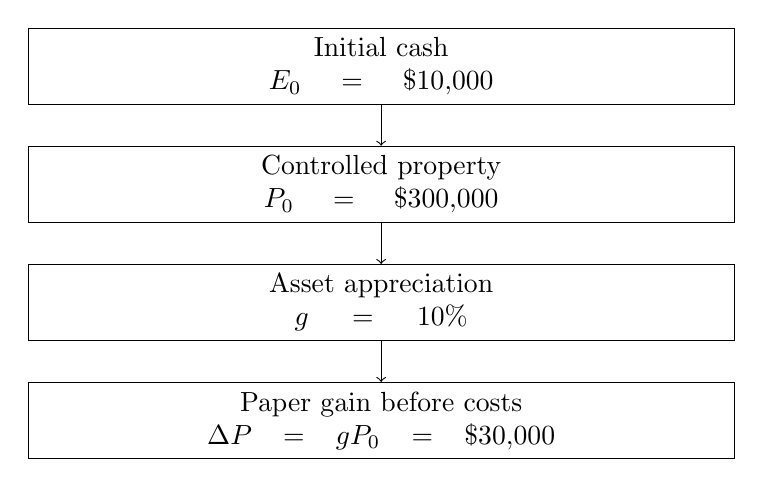
\begin{tikzpicture}
\node[draw, align=center, text width=0.72\linewidth] (cash) at (0,0) {Initial cash\\ \(E_0=\$10{,}000\)};
\node[draw, align=center, text width=0.72\linewidth] (asset) at (0,-1.5) {Controlled property\\ \(P_0=\$300{,}000\)};
\node[draw, align=center, text width=0.72\linewidth] (gain) at (0,-3.0) {Asset appreciation\\ \(g=10\%\)};
\node[draw, align=center, text width=0.72\linewidth] (paper) at (0,-4.5) {Paper gain before costs\\ \(\Delta P=gP_0=\$30{,}000\)};
\draw[->] (cash) -- (asset);
\draw[->] (asset) -- (gain);
\draw[->] (gain) -- (paper);
\end{tikzpicture}
\caption{The opening leverage mechanism: a small cash position controls a larger asset, so an asset-level gain can be large relative to the cash down payment.}
\end{figure}

\section{Time Turns a Deal Into an Asset Base}

The speaker next shifts from one-year arithmetic to a multi-decade horizon. He recalls a person who bought a property for \(\$11{,}000\) and, roughly \(60\) years later, received an offer for \(\$3{,}000{,}000\). This is an anecdote, not a forecast. Still, the scale of the comparison is useful:

\begin{equation}
M
=
\frac{\$3{,}000{,}000}{\$11{,}000}
\approx 272.7.
\end{equation}

If we annualize that multiple only as a reconstruction, the implied growth rate would satisfy

\begin{equation}
1+r
=
\left(\frac{3{,}000{,}000}{11{,}000}\right)^{1/60},
\qquad
r \approx 9.8\%.
\end{equation}

That calculation should remain secondary. The speaker's real point is not a compounding theorem. It is that the asset class rewards patience when the original purchase was sound and the owner survives the carrying costs. He also says that real estate does not go to zero in the way a stock or a business might.

We should preserve that as a practical claim, not as a universal law. A building or parcel may retain residual use value, but a particular investment can still be damaged by bad financing, repairs, vacancy, legal problems, taxes, or overpayment. The cleaner mechanism is this: buy below value, use leverage carefully, and let time work only after the deal can survive the costs of ownership.

\section{The Brokerage as Shared Infrastructure}

The lecture then pivots from investment logic to the office itself. This is not filler. The tour shows the operating structure that makes the opening claims repeatable.

The office is described as open to agents. They can work there, hold events, and use the space. The firm has moved into a newer Austin office while keeping a Round Rock office. They do not own the newer office, but they say they have a first right of refusal to buy it. That right is a piece of optionality: if another buyer appears, they get the opportunity to step in.

The tour continues through open rooms, training rooms, and daily classes. The office becomes more than a cost center. It is a platform where agents gather, learn, cold call, find opportunities, and bring deals into the firm's orbit. In compact form,

\begin{equation}
\text{space}+\text{training}+\text{access}+\text{relationships}
\longrightarrow
\text{deal flow}.
\end{equation}

This is an operating identity rather than a physical equation. It says that the brokerage is not only a place where commissions are split. It is also a machine for increasing the number of people who can recognize and act on value.

\section{From Commissions to Partnership and Equity}

The next natural question is about progression. How does an agent move from earning commissions to partnering on ownership? The answer returns to the phrase ``finding value.'' The speaker says agents do not have to spend two years making commissions before buying real estate with the brokerage. If they find the opportunity now, the brokerage can help buy it, show the process, give equity, create a new entity, and build from there.

\subsection{Question \& Answer}

What happens when a new agent can see value but cannot yet take the deal down?

The speaker answers by remembering his own obstacle. At \(24\), he could see value in a property, but his broker did not do commercial real estate. Looking back, he says he could have raised capital or brought on partners, but he did not know how to do that when he was starting.

The brokerage is presented as the missing structure. It supplies knowledge, partners, capital pathways, and entity formation. The mechanism is not merely encouragement; it is a sequence of conversion from found value to shared equity.

\begin{figure}
\centering
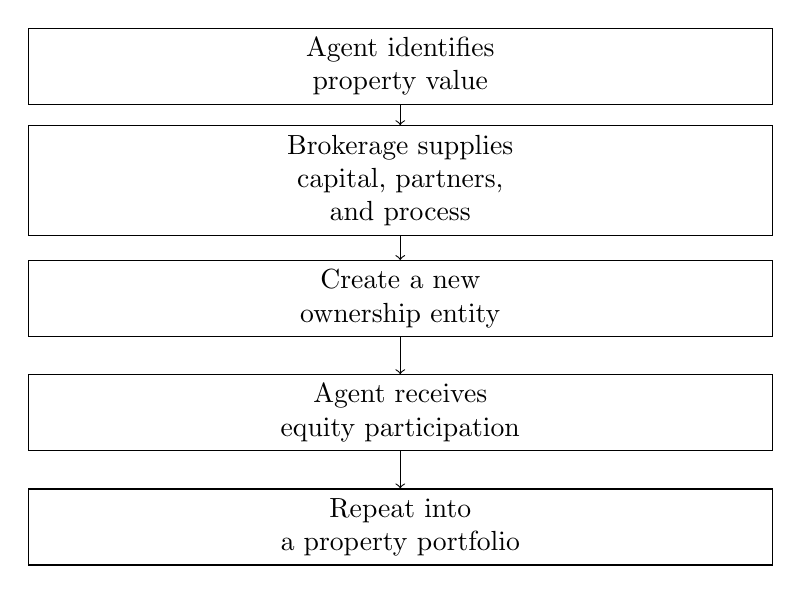
\begin{tikzpicture}
\node[draw, align=center, text width=0.76\linewidth] (agent) at (0,0) {Agent identifies\\ property value};
\node[draw, align=center, text width=0.76\linewidth] (support) at (0,-1.45) {Brokerage supplies\\ capital, partners,\\ and process};
\node[draw, align=center, text width=0.76\linewidth] (entity) at (0,-2.95) {Create a new\\ ownership entity};
\node[draw, align=center, text width=0.76\linewidth] (equity) at (0,-4.40) {Agent receives\\ equity participation};
\node[draw, align=center, text width=0.76\linewidth] (portfolio) at (0,-5.85) {Repeat into\\ a property portfolio};
\draw[->] (agent) -- (support);
\draw[->] (support) -- (entity);
\draw[->] (entity) -- (equity);
\draw[->] (equity) -- (portfolio);
\end{tikzpicture}
\caption{The agent partnership model reconstructed from the transcript: found value becomes actionable when the platform supplies capital, partners, process, and ownership structure.}
\end{figure}

This is the second form of leverage in the lecture. The first was financial leverage: cash controls property. The second is institutional leverage: a platform lets a less experienced agent act on a deal that would otherwise exceed their capital or knowledge.

\section{Culture, Sales, and the Cost of Ownership}

The interviewer then asks what separates this brokerage from more corporate or cutthroat firms. The answer is cultural, but it has a business structure behind it. In the speaker's framing, many brokerages push agents toward more commissions. This firm asks what the agent is really trying to build and how the firm can support it.

The menu is deliberately wide: build a brand, build a team, wholesale, buy real estate, or make commissions. The real estate license is one tool, not the whole identity. That distinction matters because the chapter is not about commission income alone; it is about moving from transaction work into ownership and entrepreneurial control.

The next scene introduces Killer Kim, who is doing cold calls. Asked for her sales advice, she answers with authenticity. She likes talking to people and tries to be herself. The lecture then places that human sales lesson beside the harder operational side of property ownership. She is described as owning \(16\) or \(17\) properties, with all but three paid off, and the conversation gives a monthly figure of about \(\$19{,}000\).

Those numbers should be kept, but not romanticized. The transcript immediately names the work behind them: foundation problems, septic problems, roofing problems, and the need to keep pushing. We can summarize the ownership burden as

\begin{align}
\text{rental ownership}
&=
\text{asset base}
+
\text{cash flow}
-
\text{repairs}
-
\text{debt service}
-
\text{management burden}.
\end{align}

That line is not pessimistic. It is the adult version of the leverage lesson. Leverage can amplify gains, but ownership also amplifies responsibility.

\section{Media as Message Leverage}

The lecture then moves from sales and property operations into marketing. The firm is building a room where agents can go live on Instagram, TikTok, Facebook, and YouTube. The stated purpose is not decoration. It is to let agents record their own content and make the message personal.

The marketing team explains the scale advantage. A live class might reach \(10\) people. A piece of social content might reach hundreds of thousands or millions. Later, in the podcast room, the goal is stated even more plainly: instead of talking to \(10\) people, talk to \(10\) million.

This is the media analogue of the opening leverage calculation. Let \(A_{\mathrm{room}}\) be the audience in a room and \(A_{\mathrm{social}}\) the audience reached through platforms. The reach multiple is

\begin{equation}
M_{\mathrm{reach}}
=
\frac{A_{\mathrm{social}}}{A_{\mathrm{room}}}.
\end{equation}

For example, if \(A_{\mathrm{room}}=10\) and \(A_{\mathrm{social}}=100{,}000\), then

\begin{equation}
M_{\mathrm{reach}}
=
\frac{100{,}000}{10}
=
10{,}000.
\end{equation}

Reach is not revenue. It is not trust, conversion, or profit by itself. But it changes the size of the opportunity surface. The same voice that could speak to a class can now become discoverable by a market.

\begin{figure}
\centering
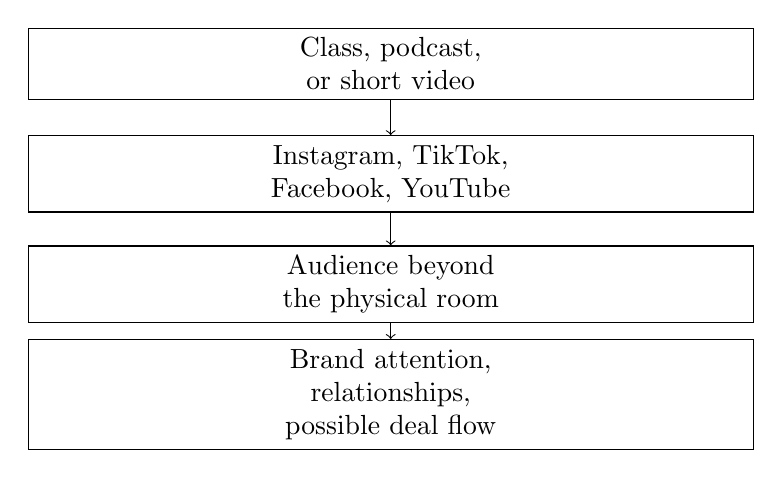
\begin{tikzpicture}
\node[draw, align=center, text width=0.74\linewidth] (class) at (0,0) {Class, podcast,\\ or short video};
\node[draw, align=center, text width=0.74\linewidth] (platforms) at (0,-1.4) {Instagram, TikTok,\\ Facebook, YouTube};
\node[draw, align=center, text width=0.74\linewidth] (audience) at (0,-2.8) {Audience beyond\\ the physical room};
\node[draw, align=center, text width=0.74\linewidth] (flow) at (0,-4.2) {Brand attention,\\ relationships,\\ possible deal flow};
\draw[->] (class) -- (platforms);
\draw[->] (platforms) -- (audience);
\draw[->] (audience) -- (flow);
\end{tikzpicture}
\caption{Media leverage: one recorded message can travel through platforms and reach an audience far larger than the room.}
\end{figure}

The Grant podcast story belongs here because it shows media becoming relationship capital. A late-night Clubhouse opening becomes an email, the email becomes a podcast booking, and the podcast becomes a business meeting. The lesson is not merely to be persistent. It is to prepare for access so that attention can be converted into a real conversation.

\section{Finding Value, Wholesaling Land, and the Machine}

The final instructional movement returns to the portable skill underneath the whole day: learn how to find value and find deals. A five-year real estate operator says that this skill matters whether one is an agent, wholesaler, investor, or capital raiser. If one can identify value and opportunity, he says, one can make money in many market conditions.

\subsection{Question \& Answer}

If someone had to start from zero and had one year to make serious money, what concrete path does the speaker choose?

He answers: wholesale land in Austin, Texas. The described process is to find good land, put it under contract at a good price, and then find a developer or end buyer willing to pay more.

Let \(P_{\mathrm{contract}}\) be the contract price and \(P_{\mathrm{end}}\) the end-buyer price. The gross spread is

\begin{equation}
S_{\mathrm{gross}}
=
P_{\mathrm{end}} - P_{\mathrm{contract}}.
\end{equation}

For the strategy to have a positive spread,

\begin{equation}
P_{\mathrm{end}} > P_{\mathrm{contract}}.
\end{equation}

This is the wholesaler's version of buying below value. The investor may not intend to own the land for decades. The value is in controlling a contract that another buyer values more highly. The transcript gives no specific land numbers, so the notes should not invent them. The structure is the spread, and the skill is finding it.

The tour then moves to Round Rock and the group meets the department head for what they call ``the machine.'' This is the call-center and lead-generation side of the brokerage. The description is practical: inbound and outbound work, reaching out to people asking about homes, connecting them with agents, and routing them through credit repair if needed, lending partners, and financing.

\begin{figure}
\centering
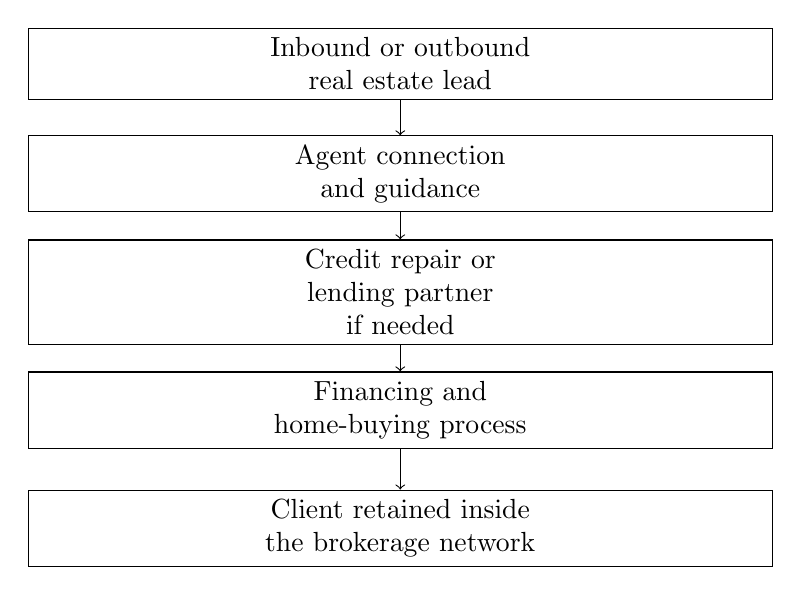
\begin{tikzpicture}
\node[draw, align=center, text width=0.76\linewidth] (lead) at (0,0) {Inbound or outbound\\ real estate lead};
\node[draw, align=center, text width=0.76\linewidth] (agent) at (0,-1.4) {Agent connection\\ and guidance};
\node[draw, align=center, text width=0.76\linewidth] (support) at (0,-2.9) {Credit repair or\\ lending partner\\ if needed};
\node[draw, align=center, text width=0.76\linewidth] (finance) at (0,-4.4) {Financing and\\ home-buying process};
\node[draw, align=center, text width=0.76\linewidth] (house) at (0,-5.9) {Client retained inside\\ the brokerage network};
\draw[->] (lead) -- (agent);
\draw[->] (agent) -- (support);
\draw[->] (support) -- (finance);
\draw[->] (finance) -- (house);
\end{tikzpicture}
\caption{The ``machine'' as described in the transcript: lead generation, routing, partner support, and an in-house client path.}
\end{figure}

This is the third form of leverage. We have seen financial leverage, where cash controls a larger property; institutional leverage, where a brokerage helps agents act on opportunities; and media leverage, where one message reaches a larger market. The machine adds process leverage. It is the attempt to make lead generation, agent assignment, and client routing repeatable.

\section{Summary}

The chapter begins with a small arithmetic puzzle and ends with a business system. The opening calculation is

\begin{equation}
R_E = \frac{gP_0}{E_0},
\end{equation}

but the transcript keeps us honest: this is paper return before costs. Time, repairs, debt, taxes, vacancy, and execution decide whether the arithmetic becomes durable wealth.

The rest of the day shows the supporting machinery. The office supplies shared infrastructure. The partnership model converts agent-found value into equity. Cold calling supplies human contact. Social media supplies reach. Wholesaling land supplies a concrete spread model. The Round Rock machine supplies a repeatable client path.

The durable lesson is not that real estate automatically creates wealth. It is that wealth is built when several forms of leverage work together: buying below value, controlling assets with disciplined equity, sharing infrastructure with agents, distributing the message through media, and building systems that create and route opportunity.